\documentclass{article}
\usepackage{graphicx}
\usepackage{hyperref}
\graphicspath{ {./images/} }
%Includes References in the table of contents%
\usepackage[nottoc]{tocbibind}
\usepackage{float}
\usepackage{amsmath}

\usepackage[square, numbers]{natbib}
\bibliographystyle{abbrvnat}

\title{Team 26: Text summarization}

\newcommand{\bertlarge}{$\text{BERT}_{LARGE}$ }
\newcommand{\bertbase}{$\text{BERT}_{BASE}$ }
\newcommand{\gptmedium}{$\text{GPT-2}_{MEDIUM}$ }
\newcommand{\gptlarge}{$\text{GPT-2}_{LARGE}$ }



\begin{document}
	
\maketitle
\maketitle

\begin{abstract}
	\noindent
	In our project, we have decided to create text summarizer with BERT. 
	There is already a Bert Extractive Summarizer -package. It's based on following article: \href{https://arxiv.org/ftp/arxiv/papers/1906/1906.04165.pdf}{https://arxiv.org/ftp/arxiv/papers/1906/1906.04165.pdf}
	This package is intended for lecture-summarization, and our goal is to extend and fine-tune this model for news or scientific articles.
	Even though foundational work is already done for the package, there's still much to customize such as tokenizer and model. 
	Our target language is english. Summarization tools such as Bilingual Evaluation Understudy (BLEU) and Recall-Oriented Understudy for Gisting Evaluation (ROUGE) are available, and part of the project is to try to evaluate the texts automatically and manually.	
\end{abstract}

\clearpage
\section{Introduction}
Automatic summarization is the process of shortening a set of data computationally, to create a subset (a summary) that represents the most important or relevant information within the original content. There are two main approaches to automatic summarization (independently of the application domain, e.g. text, images, video etc.):
\begin{itemize}
	\item Extraction-based or extractive summarization 
	\item Abstraction-based or abstractive summarization
\end{itemize}

When it comes to text documents, summarization is closely related to data compression and information understanding. The ability to produce coherent, well-structured summaries has the potential to transform efficiently the way that discovery systems work, as well as help human readers in skimming large datasets of text documents. That is why automatic summarization is considered one of the most important, yet least solved, tasks in NLP and a method that will transform the way people consume information on the Internet. In conclusion, applying text summarization reduces reading time, accelerates information retrieval and increases the amount of useful, dense information. In our case, we will deal with extractive summarization where a system produces summaries by choosing a subset of the initial text.

\section{Background}
The first summarization techniques go back already more than 50 years to Luhn’s and Edmundson’s seminal papers on automatic summarization (1958 and 1969 respectively, \cite{textmining1958}, \cite{automaticextracting}). Early work in the field dealt with single document summarization (news story, scientific articles etc.) Later, multi document summarization was applied in big data clusters to provide a coherent and brief digest to the users. \\



\section{Methods}


\section{Experiments}



\section{Results}

Evaluation was done on newsroom dataset \cite{dataset}. The model inference however is extremely slow, and only a subset of samples was chosen to be evaluated. The sample size was chosen to be 500 at randomly, which resulted in tolerable running times (< 60 minutes). 

\subsection{General text properties}

\noindent
Two different BERT models were tested, \bertlarge and \bertbase. These models were compared against baseline model Lede-3 and GPT-2. GPT-2 was chosen to be compared against BERT models, because in the original study \cite{extractive_bert} they noticed that BERT should be generating more representative embeddings of the sentences. Also \gptlarge was chosen as one model to be evaluated. \gptlarge has 774 million parameters, which is roughly the double of parameters in \bertlarge and \gptmedium. Also GPT-2-XL and new GPT-NEO (GPT-3 replication) would've been interesting comparisons, but unfortunately they were too large to fit on GPU.\\

\noindent
The python package bert-extractive-summarizer \cite{extractive_bert} uses only sentences from original text, and the amount of sentences is defined by either fixed ratio, or amount of sentences. In this case the ratio was defaulted to 0.2, which means that we use 20\% of the sentences from original text. We can calculate empirical distribution of the ratios seen in reference summaries as displayed in Figure \ref{fig:empirical_ratio}.


\noindent
\begin{figure}[H]
	\centering
	\hspace*{-3cm}
	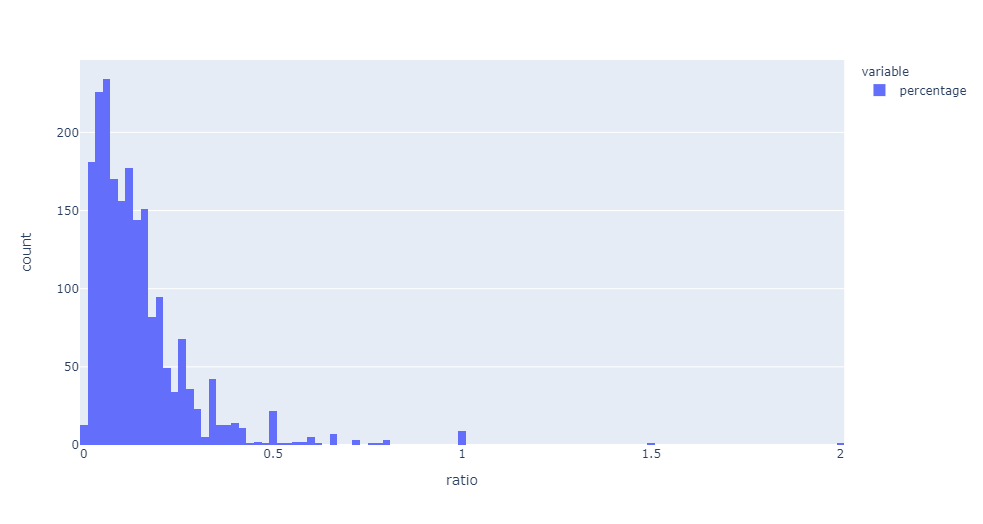
\includegraphics[scale=0.55]{empirical_ratio.png}
	\caption{Distribution of observed ratios in the data}
	\label{fig:empirical_ratio}
\end{figure}

\noindent
Here we can see that the mean is around 0.15. We can also plot what length of sentences there are as in following Figure \ref{fig:empirical_lengths}.

\noindent
\begin{figure}[H]
	\centering
	\hspace*{-3cm}
	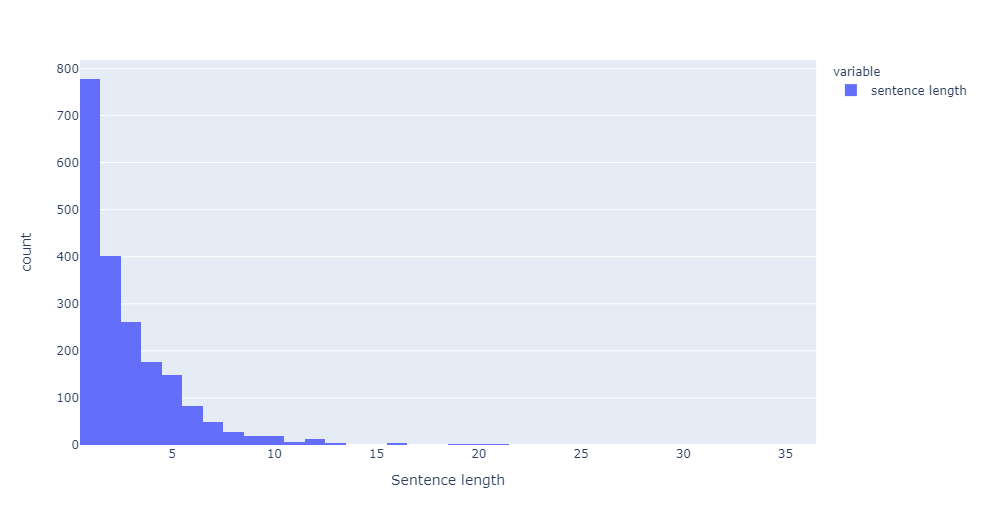
\includegraphics[scale=0.55]{empirical_lengths.png}
	\caption{Distribution of observed ratios in the data}
	\label{fig:empirical_lengths}
\end{figure}

\noindent
Here we actually see that there are multiple summaries which have sentence amount of 1. This is important to remember because it might favor Lede-3 classifier due to shortness of text, as we see later.\\

\noindent
We can also view the actual summary distribution statistics from the dataset website summari.es \cite{dataset}. By using their visualization tool, we get following distribution. \\

\noindent
\begin{figure}[H]
	\centering
	\hspace*{-3cm}
	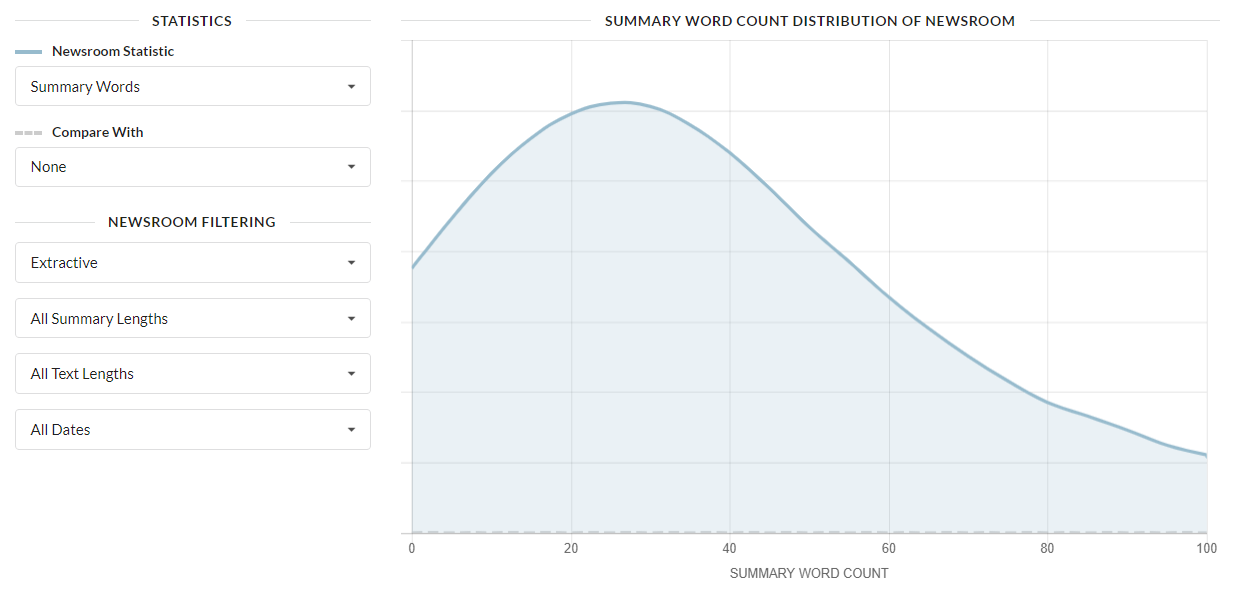
\includegraphics[scale=0.55]{words_in_summary.png}
	\caption{Distribution of words in summaries}
	\label{fig:words_in_summary}
\end{figure}

\noindent
If we plot amount of words seen in our samples, we get similar looking plot as in following Figure.\\

\noindent
\begin{figure}[H]
	\centering
	\hspace*{-3cm}
	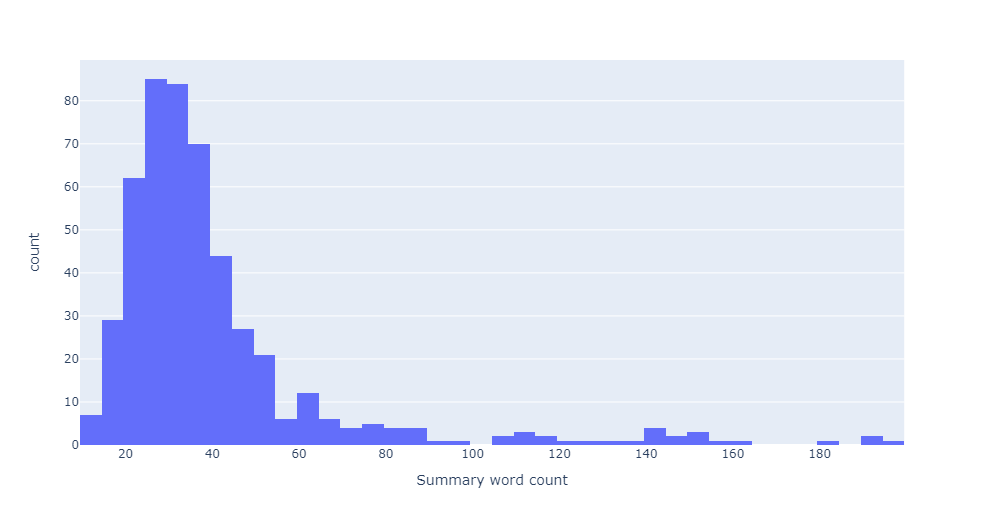
\includegraphics[scale=0.55]{empirical_summary_words.png}
	\caption{Distribution of words in summaries}
	\label{fig:empirical_summary_words}
\end{figure}

\noindent
From this it seems that newsarticle summaries tend to be short.\\

\subsection{Recall-Oriented Understudy for Gisting Evaluation (Rouge)}

ROUGE is a metric which determines the quality of summary. In this experiment we used ROUGE-N and ROUGE-L metrics. ROUGE-N metric measures n-gram overlapping between generated and reference summaries. ROUGE-L metric compares the longest common subsequence between generated and reference summaries. ROUGE recall can be defined as following \cite{rouge}: \\

\begin{align*}
	\text{ROUGE-recall} &= \dfrac{\text{n-overlapping-words}}{\text{n-words-in-reference-summary}}
\end{align*}\\

\noindent
and ROUGE precision as following:\\

\begin{align*}
	\text{ROUGE-precision} &= \dfrac{\text{n-overlapping-words}}{\text{n-words-in-generated-summary}}
\end{align*}\\

\noindent
ROUGE-f1 score used in the coding implementation is similar to normal f1-scores, this time just used with ROUGE-precision and ROUGE-recall. \cite{rouge}\\

\noindent
Rouge scores seem to be dominated by Lede-3. Lede-3 is known to have strong performance, comparable with state-of-art methods as discussed in \cite{dataset}. Otherwise the models are performing similarly, although \gptmedium is achieving slightly higher scores. All of the rouge scores are seen in Figures \ref{fig:rouge1_02}, \ref{fig:rouge2_02} and \ref{fig:rougel_02} below. 

\begin{figure}[H]
	\centering
	\hspace*{-3cm}
	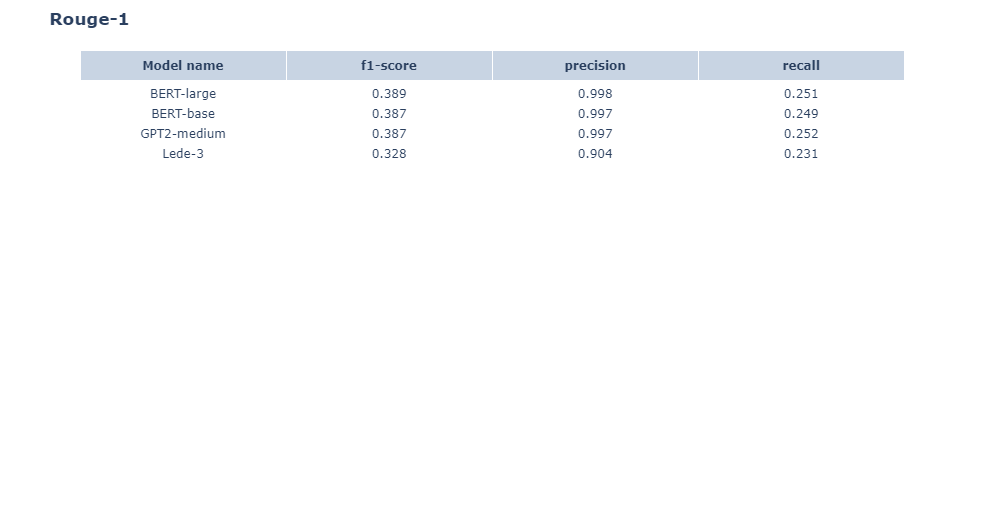
\includegraphics[scale=0.55]{rouge1.png}\\
	\caption{Rouge-1 scores with ratio=0.2}
	\label{fig:rouge1_02}
\end{figure}

\begin{figure}[H]
	\centering
	\hspace*{-3cm}
	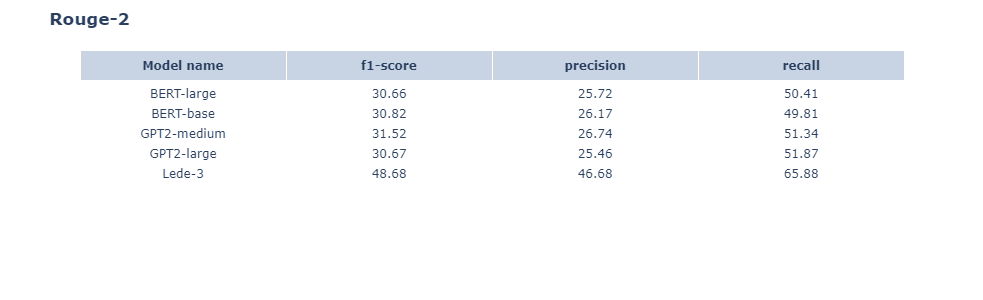
\includegraphics[scale=0.55]{rouge2.png}\\
	\caption{Rouge-2 scores with ratio=0.2}
	\label{fig:rouge2_02}
\end{figure}

\begin{figure}[H]
	\centering
	\hspace*{-3cm}
	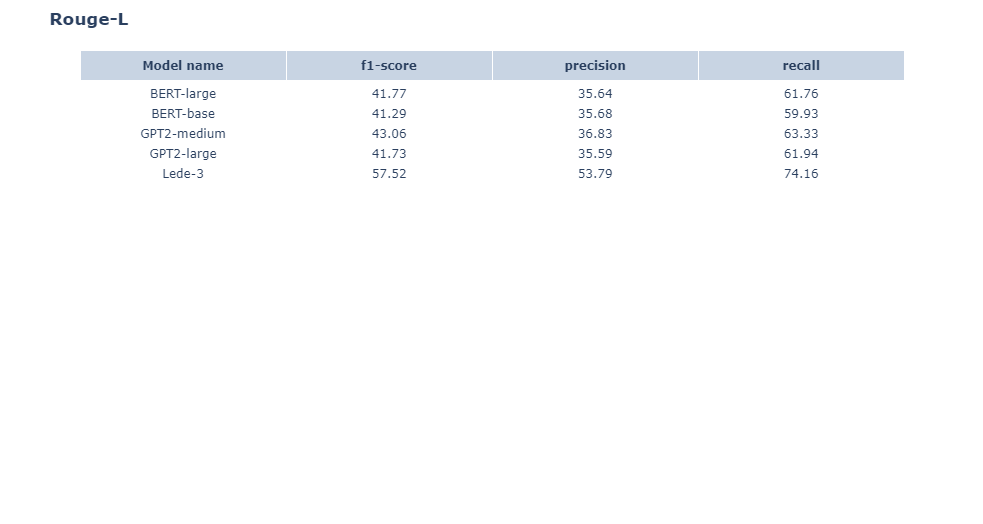
\includegraphics[scale=0.55]{rougel.png}\\
	\caption{Rouge-L scores with ratio=0.2}
	\label{fig:rougel_02}
\end{figure}

\subsection{Bilingual Evaluation Understudy (BLEU)}

\noindent
We can also take a look at BLEU scores for each model. BLEU measures how much the n-grams in our generated summary appears on the reference summaries. BLEU performs similarly to ROUGE-precision, except BLEU introduces brevity penalty, which penalizes generated summaries that are shorter than reference summaries. As Lede-3 summaries are always of length 3, we can see how much Lede-3 is actually punished by looking at how many summaries have 3 sentences or more from the summary distribution in Figure \ref{fig:empirical_lengths}. We see that majority of the sentences are under 3. This means that Lede-3 sentences are not punished, and it actually provides really good performance on this dataset. 

\begin{figure}[H]
	\centering
	\hspace*{-2cm}
	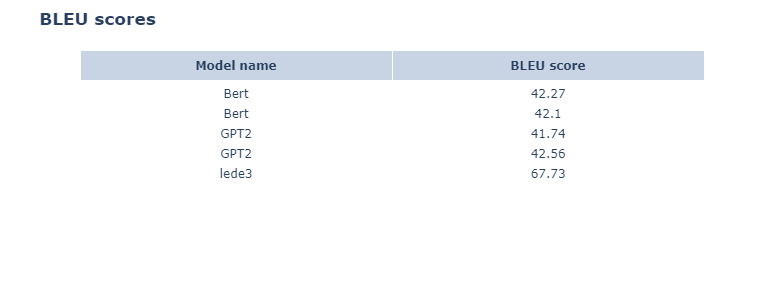
\includegraphics[scale=0.55]{bleu_scores.png}\\
	\caption{BLEU scores with 4-grams}
	\label{fig:bleu}
\end{figure}


\section{Discussion}

\noindent
In this experiment we saw how well extractive text summarization works if we choose sentences based on their centrality. For this we used K-means clustering to cluster embeddings that achieved from BERT-models. We used Lede-3 as baseline, and compared GPT-models to see how well they produce embeddings. We found out that Lede-3 acually is the most accurate summarization technique in this sense. Although Lede-3 is very simple algorithm and it has no understanding of the underlying text, it seems like the texts are written in such way that first sentences produce most important aspects of the text. This is interesting realization, and in the future it would be interesting to try to fine tune some deep learning model to see, whether it actually is able to outperform Lede-3 or not.\\

\noindent
In this experiment it was also interesting to see how four state-of-art models performed when extracting embeddings without fine tuning. Most interesting note was that scaling the model (\gptlarge) didn't necessarily result in better embeddings with respect to our task. \\

\noindent
This clustering approach was used when summarizing lecture videos in \cite{extractive_bert}, where this approach is more viable because lectures aren't as well structured as news articles. 


\section{Division of labor}


\section{Appendix}

% Import bibliography file %
\bibliography{citations/sources.bib}

\end{document}

